\documentclass[10pt,a4paper]{scrartcl}
\pagestyle{empty}
\usepackage{a4} % alternativ \usepackage{a4wide}
\usepackage[ngerman]{babel} % Neudeutsche Silbentrennung (mehrsprachiges Dokument)
\usepackage{parskip} % Skip indentation of first row
\usepackage{graphicx} % Graphics support
\usepackage{longtable} % Tables across several pages
\usepackage{booktabs}
\usepackage{hyperref} % Hyperlinks
\usepackage{float} % Force float position
\usepackage[automark]{scrpage2} %kopf/fusszeile
\usepackage[utf8x]{inputenc} % Unicode-Encoding
 
\restylefloat{figure} % Force float position
\linespread{1.3}

\author{Danilo Bargen, Christian Fässler, Jonas Furrer} 
\title{Software Architektur Dokument\\ Projekt BierIdee}

\pagestyle{scrheadings}
\ihead{SE2 Projekte} %linke Kopfzeile
\ohead{BierIdee} %rechte Kopfzeile

\begin{document}

\begin{titlepage}
	\maketitle
	\vspace{120mm}
	\thispagestyle{empty} % Don't start page numbers on this page
\end{titlepage}

\tableofcontents
\newpage

\section*{Änderungshistorie}
\begin{tabular}{p{0.1\textwidth}p{0.15\textwidth}p{0.55\textwidth}p{0.1\textwidth}}
\toprule
\textbf{Version} & \textbf{Datum} & \textbf{Änderung} & \textbf{Person} \\  
\midrule
v1.0 & 02.04.2012 & Dokument erstellt & dbargen \\  
\hline 
v1.1 & 05.05.2012 & Frontendarchitekturdiagramm & dbargen \\  
\hline 
v1.2 & 05.05.2012 & Dokument überarbeitet & dbargen \\  
\bottomrule
\end{tabular} 
\newpage

\section{Einführung}

\subsection{Zweck}
Dieses Dokument beschreibt die Softwarearchitektur des Projektes BierIdee.

\subsection{Gültigkeitsbereich}
Die Gültigkeit des Dokumentes beschränkt sich auf die Dauer des SE2-Projekte Modules FS2012.

\subsection{Referenzen}

\begin{itemize}
	\item REST.Interface.pdf
	\item Evaluation.Datenbank.pdf
	\item Authentication.pdf
\end{itemize}

%\bibliographystyle{alpha}
%\bibliography{SoftwareArchitekturDokument}

\subsection{Übersicht}

Das System der Bieridee kann in drei Kategorien/Teilbereiche unterteilt werden: Die Datenbank, die
REST API und die Clientanwendung. Zwischen der API und der Android-Clientanwendung wird
ausschliesslich via HTTP kommuniziert. Um auf die API zuzugreifen, muss man sich mit einem
API-Token authentifizieren und die Requests mit einem kryptografischen Verfahren signieren. 
Logisch werden im Backend die Datenbank- und API-bezogenen Klassen in einem gemeinsamen Package
geführt. Das Frontend wird nach dem MVC Pattern und gemäss Android Best Practices implementiert. 
Beim Deployment wird die API direkt über den eingebauten Webserver von Restlet gestartet, ohne
Servlet-Container. Es wird aber aus Performance- und Optimierungsgründen ein Reverse Proxy
davorgesetzt. Alle Daten werden im Backend persistent in einer Graphendatenbank gespeichert und
durch Traversierung und eingebaute Algorithmen abgefragt. Das System soll in der Testphase bis zu
50 gleichzeitige Nutzer bedienen können.


\newpage
\section{Systemübersicht}
Unsere Systemarchitektur gliedert sich in drei Teilbereiche: Die Datenbank, die REST API
und die Clientanwendung.

\begin{figure}[H]
	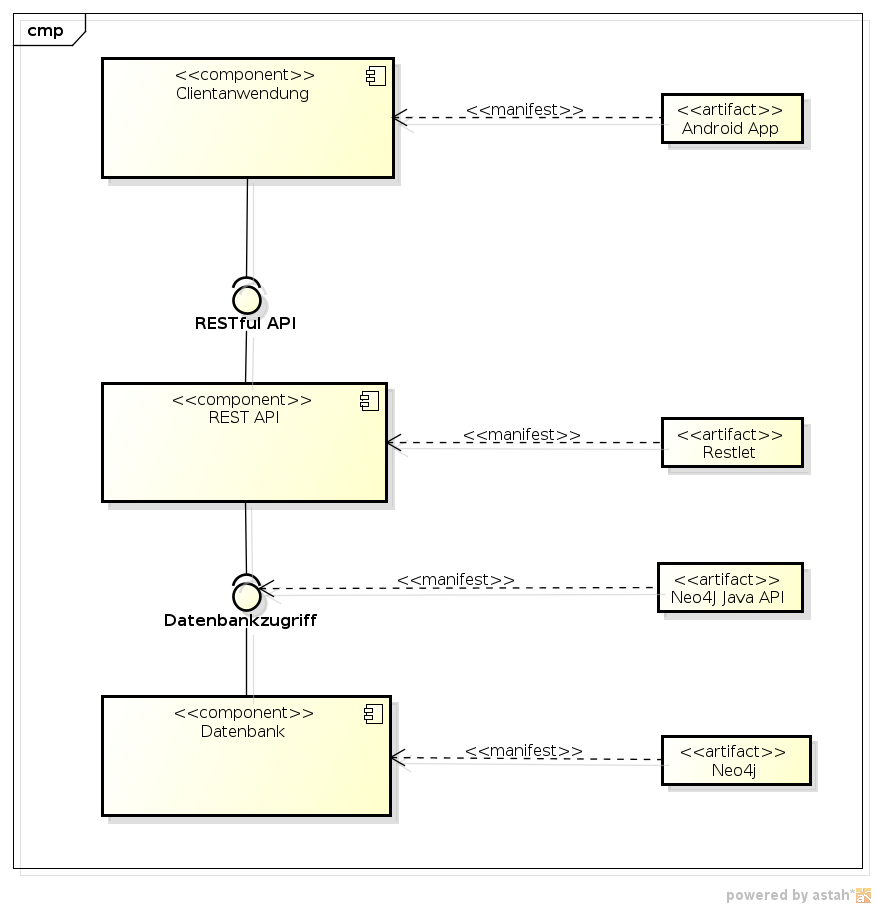
\includegraphics[width=\textwidth]{ComponentDiagram.png}
	\caption{Komponentendiagramm}
	\label{fig:component_diagram}
\end{figure}


\subsection{Komponenten}

\subsubsection{Datenbank}

Als Datenbank kommt die Graphendatenbank Neo4j\footnote{\texttt{http://neo4j.org/}} zum Einsatz.
Eine Graphendatenbank hat den Hauptvorteil, dass man sehr gut mit den Relationen arbeiten kann und
so beispielsweise die Bier-Empfehlungen durch Traversierung realisieren kann. Näheres zum Entscheid
zur Verwendung einer Graphendatenbank siehe Dokument Evaluation.Datenbank.pdf

\subsubsection{REST API}

Für das Zwischenglied zwischen Daten und Client kommt ein
RESTful\footnote{\texttt{http://en.wikipedia.org/wiki/Representational\_state\_transfer\#RESTful\_web\_services}}
Web Service zum Zuge. Diese REST API wird mithilfe von
Restlet\footnote{\texttt{http://www.restlet.org/}} realisiert. Die Domainobjekte werden in Form von
abstrakten Ressourcen mit entsprechenden Repräsentationen zur Verfügung gestellt.

Die REST-Ressourcen werden im Dokument \textit{REST.Interface.pdf} näher spezifiziert.

\subsubsection{Clientanwendung}

Die Android Clientanwendung greift auf die REST API zu und stellt die Informationen auf sinnvolle
Art und Weise dar.


\subsection{Schnittstellen}

\subsubsection{Datenbankzugriff}

Der Datenbankzugriff geschieht über die eingebaute Java-Schnittstelle von Neo4j. Dadurch wird die
Verwendung von JDBC oder eines OR Mappers unnötig. Datenbanknodes können entweder via
objektorientierter Syntax oder mithilfe einer domainspezifischen Abfragesprache namens
\textit{Cypher} abgefragt werden.

\subsubsection{REST API / HTTP}

Die RESTful API wird von Restlet bereitgestellt. Die Domainobjekte werden in Ressourcen gegliedert
und via HTTP im JSON- oder XML-Format ausgegeben.


\section{Architektonische Ziele \& Einschränkungen}

\subsection{Safety / Security}

Die API wird nicht öffentlich/frei zugreifbar sein. Das Sicherheitskonzept ist zweistufig aufgebaut.
Einerseits erzeugt die API sogenannte API-Tokens, mit welchem sich die App als "`trustful"' App
identifiziert.

In einem zweiten Schritt authentifiziert und autorisiert sich der Benutzer der Android App mittels
Benutzernamen und Passwort-Hash. Die Daten werden jedoch nicht direkt übertragen, sondern werden nur
benutzt um die Requests mithilfe des HMAC-SHA256 Verfahrens zu signieren.

Das genaue Authentifizierungs bzw. Signierungsverfahren ist im Dokument Authentication.pdf dokumentiert.

\paragraph*{Security-Steps:}

\begin{enumerate}
	\item App Authentifizierung mittels App-Token
	\item User-Authentifizierung mittels Benutzername und Passwort
	\item Autorisierung für gewünschte Operationen
\end{enumerate}
 
Alle Schritte werden bei jeder Anforderung einer Ressource (http Request) durchgeführt, um das
Prinzip der \textit{Statelessness} von RESTful APIs zu gewährleisten.

Auf Datenbankebene wird kein Rechtesystem implementiert. Die Datenbank ist auch nicht direkt
ansprechbar, daher kann das ganze Berechtigungssystem in der REST API realisiert werden.


\section{Logische Architektur}

Die grundsätzliche Aufteilung in Subsysteme in diesem Projekt wird bereits im Kapitel
\textit{Systemübersicht} beschrieben, deshalb wird hier primär auf die Package-Architektur
eingegangen.

Die logische Architektur des Gesamtprojektes wird in zwei Hauptkategorien bzw. Packages unterteilt --
\textit{android} und \textit{back}. Beide Packages sind Unterpackages von
\textit{ch.hsr.bieridee}.

Im nachfolgenden Diagramm sieht man die Aufteilung der Projektteile in Packages.

\begin{figure}[H]
	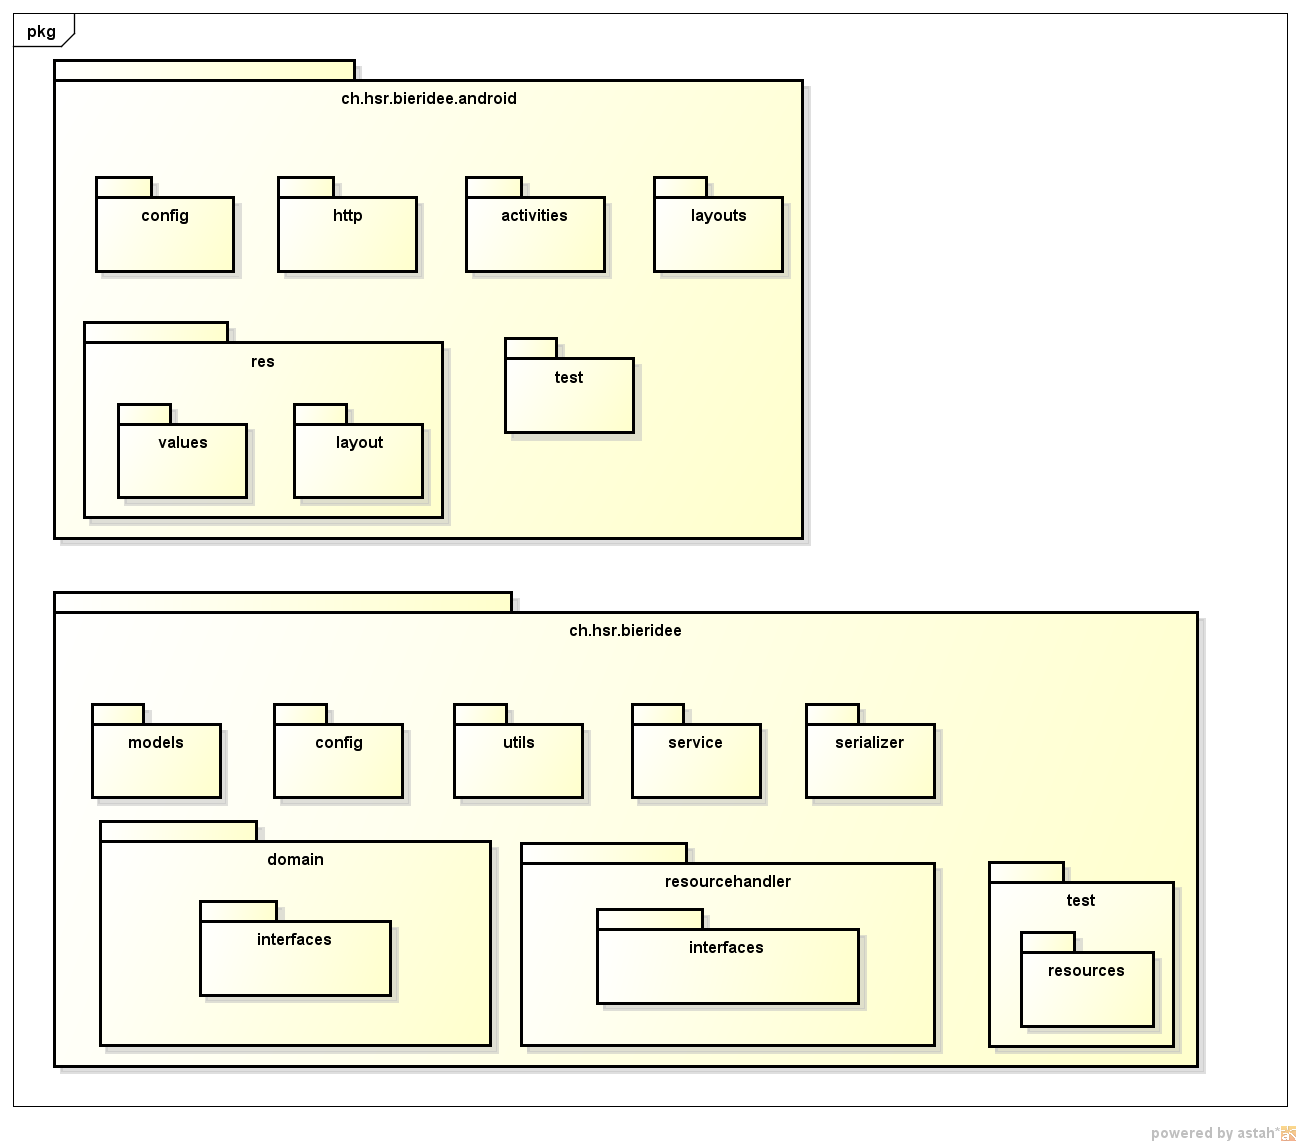
\includegraphics[width=\textwidth]{PackageDiagramm.png}
	\caption{Package Diagramm}
	\label{fig:package_diagram}
\end{figure}

Selbstverständlich wird die Android-Applikation nach dem Model-View-Controller Modell implementiert.
Dies ist jedoch zusammen mit dem Ressourcen-Management (Templates, Strings, Grafiken etc) ein
integraler Bestandteil des Android SDKs, deshalb wird es hier nicht genauer erörtert.


\newpage
\section{Backend Architektur}

Die Backend-Architektur ist ein ziemlich wichtiger Teil des Architekturdokumentes. Deshalb
nachfolgend ein detailliertes Backend-Architektur-Klassendiagramm am Beispiel eines Bier-Objektes.

\begin{figure}[H]
	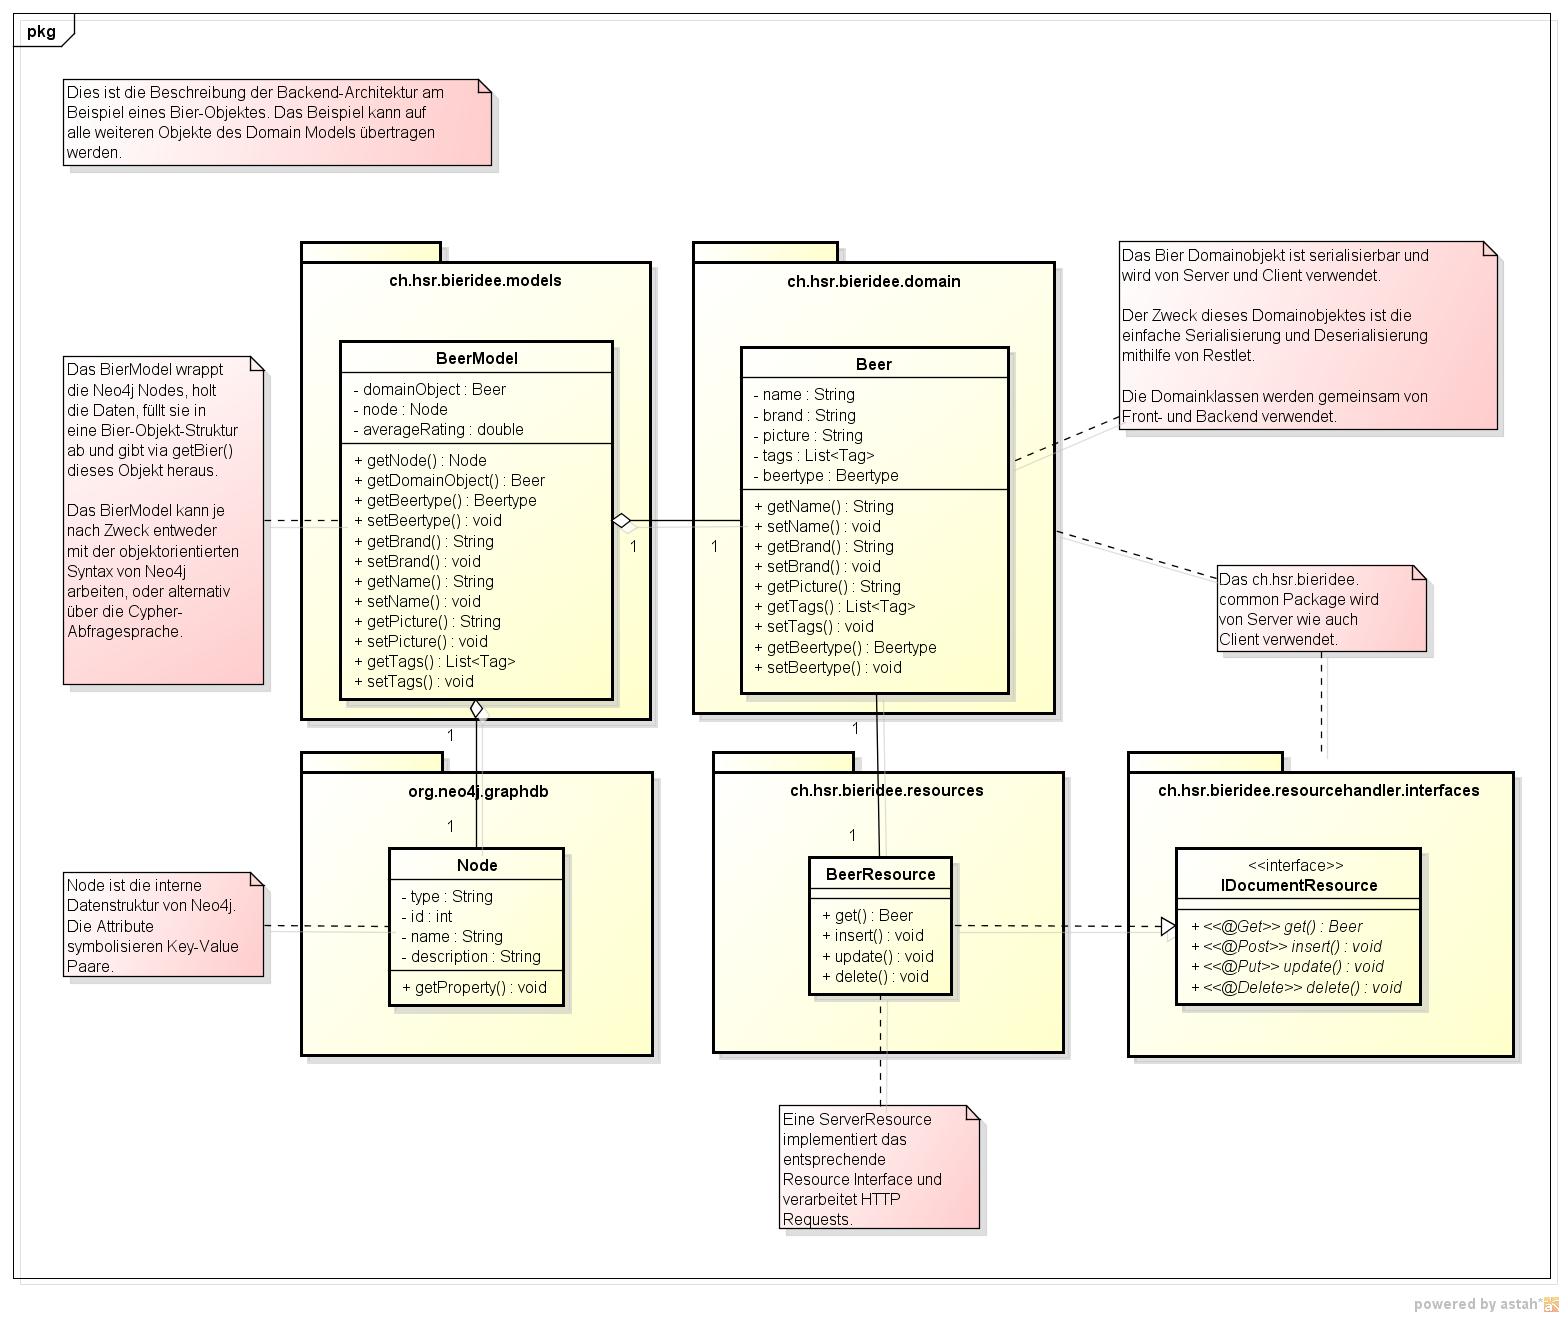
\includegraphics[height=\textwidth,angle=90]{BackendArchitektur.png}
	\caption{Backend Architektur}
	\label{fig:backend_architecture}
\end{figure}

\newpage
\section{Frontend Architektur}

Dieses Diagramm zeigt einen Ausschnitt aus der Frontendarchitektur am Beispiel der Bierliste. Die
Architektur ist grösstenteils durch das Android SDK und ihre Best-Practice Richtlinien vorgegeben.

\begin{figure}[H]
	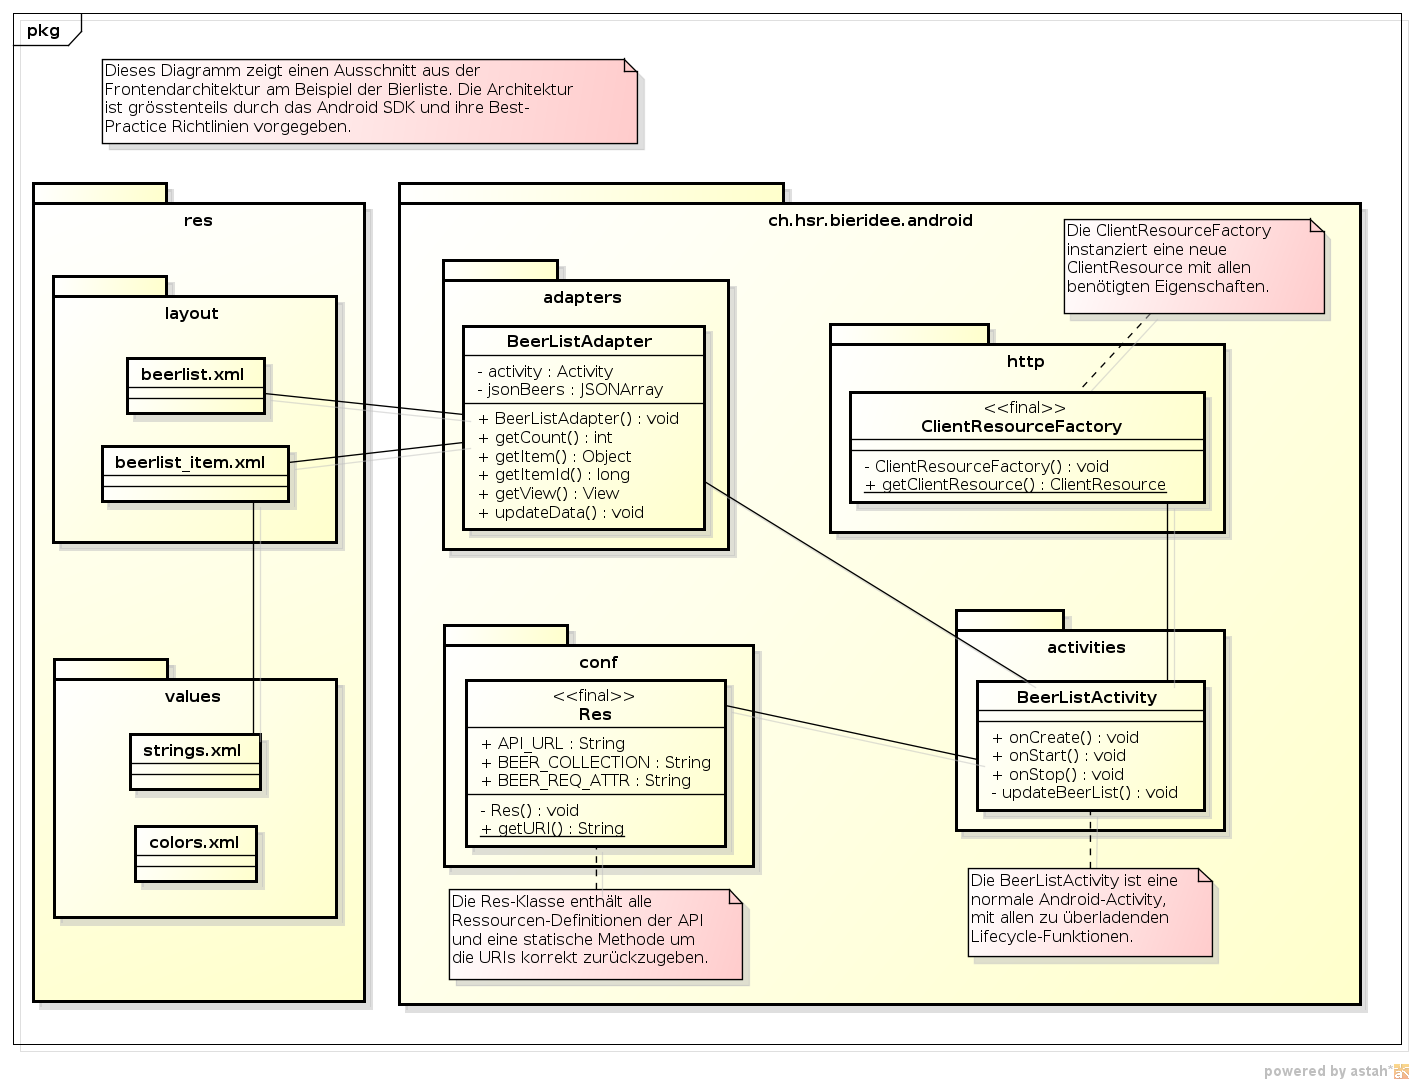
\includegraphics[height=\textwidth,angle=90]{FrontendArchitektur.png}
	\caption{Frontend Architektur}
	\label{fig:frontend_architecture}
\end{figure}


\section{Prozesse und Threads}

\subsection{Datenbank}

Die Neo4j Datenbank garantiert die ACID Prinzipien.
Sämtliche Datenzugriffe erfolgen in Transaktionen, somit ist die Integrität der Datenbank
sichergestellt.
Neo4j ist komplett thread safe implementiert.  Die Datenbank wird im
embedded Modus verwendet und kann direkt über eine Java API angesprochen werden.

\subsection{Server API}

Die Server API ist multithreaded. Für jede Clientanfrage wird ein Worker Thread erstellt welcher den
Request bearbeitet.

Die benötigten Ressourcen-Handler werden bei jeder Anfrage neu instanziert, somit müssen diese
Komponenten nicht thread safe implementiert sein.

\subsection{Android App}

Die UI ist single threaded. Langlaufende Operationen werden in asynchrone Background-Threads ausgelagert und
benachrichtigen das UI mithilfe von Callbacks.


\section{Deployment}

\begin{figure}[H]
	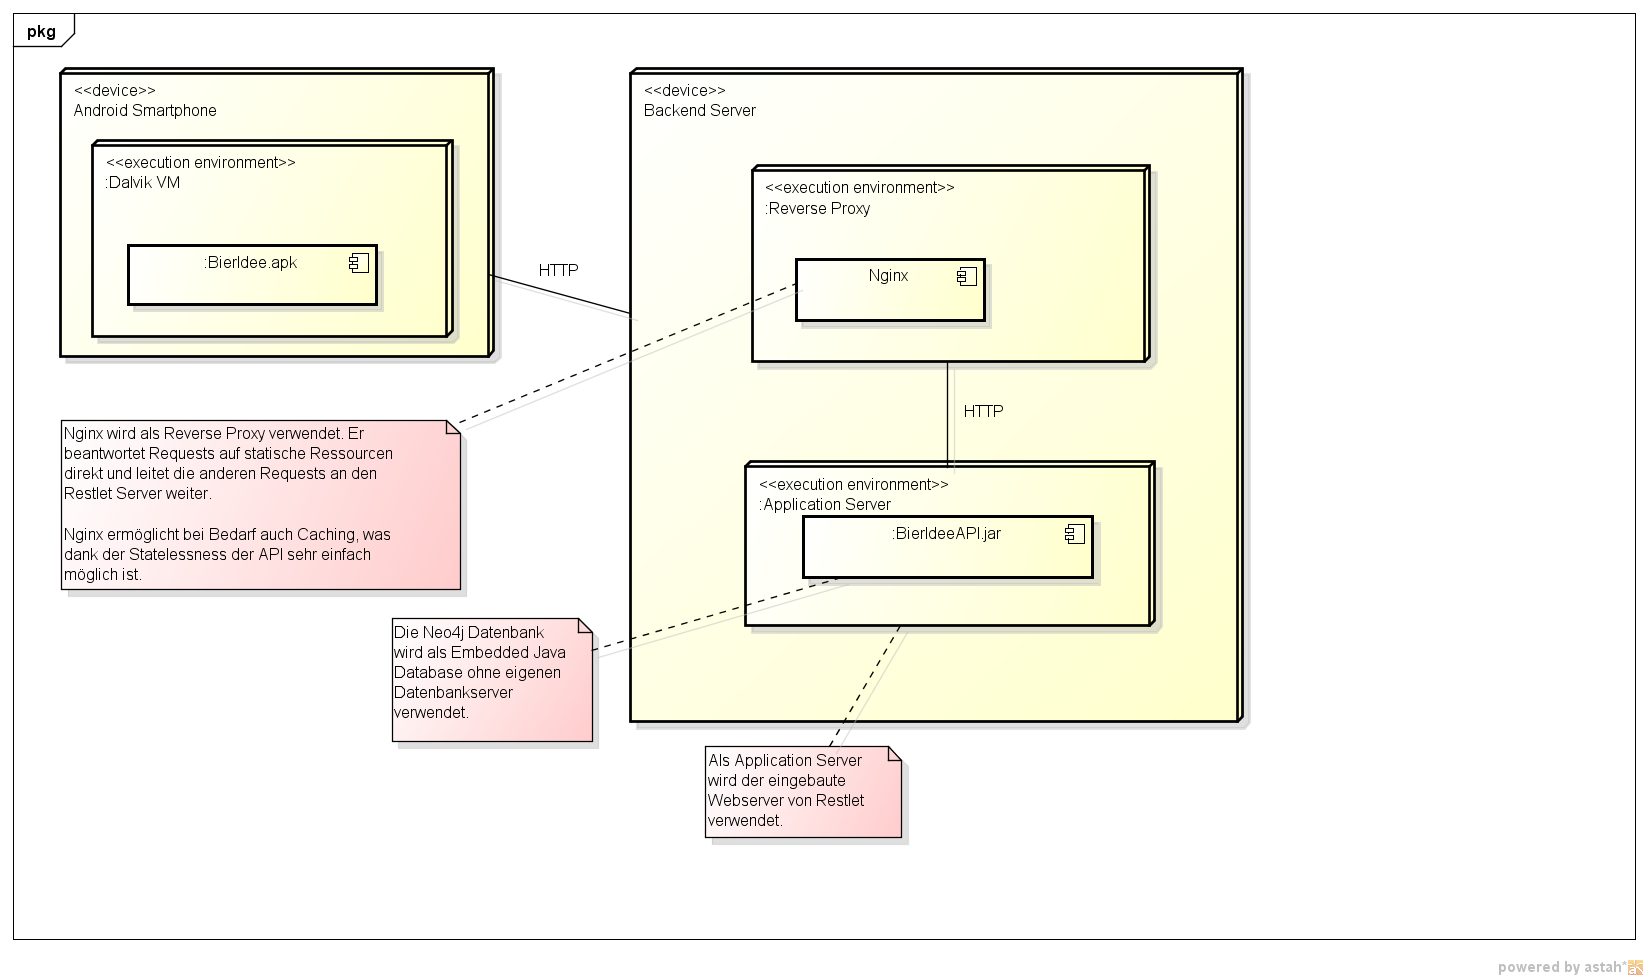
\includegraphics[width=\textwidth]{DeploymentDiagram.png}
	\caption{Deployment Diagramm}
	\label{fig:deployment_diagram}
\end{figure}

\subsection{Frontend}

Die Frontend-Applikation wird im Rahmen dieses Projektes manuell als \texttt{.apk}-Datei auf die
Testgeräte kopiert werden. Falls das Projekt weitergezogen wird, wäre eine Publikation im Android
Market gut denkbar, für den Moment wird aber darauf verzichtet.


\subsection{Backend}

Das Backend wird auf einem Debian Linux Server deployed. Die Application Server Instanz läuft
mithilfe von Java 1.6 und Restlet ohne zusätzliche Software.

Zur Überwachung des Systemprozesses
wird Supervisor verwendet (nicht im Deployment Diagramm erwähnt, da kein integraler Bestandteil).
Supervisor überwacht den Systemprozess und startet ihn, falls er abstürzt, sofort neu. 

Vor den Application Server wird ein Reverse Proxy -- konkret Nginx -- gesetzt. Dieser nimmt alle
Requests entgegen und entscheidet, ob es sich dabei um statische oder um dynamisch generierte Daten
handelt. Statische Daten -- beispielsweise Bilder -- werden direkt zurückgeliefert, während
die anderen Requests an den Application Server weitergegeben werden. So kann auch ein Caching
problemlos implementiert werden, was den Application Server entlastet und die Skalierbarkeit stark
erhöht.


\section{Datenspeicherung}

Die Daten werden in einer Graphendatenbank (konkret Neo4j) abgelegt. Diese besteht grundsätzlich nur
aus zwei Arten von Objekten -- Nodes und Relationen. Mithilfe von diesen zwei Objekten kann die
gesamte Datenstruktur sehr flexibel abgebildet werden; Abfragen können mit gezielter Traversierung
durch eine domainspezifische Abfragesprache namens \textit{Cypher} ausgedrückt werden.

Der Evaluationsbeschrieb der Datenbank findet sich im Dokument \textit{Evaluation.Neo4j.pdf}.

Nachfolgend das allgemeine Datenbankdiagramm sowie ein Diagramm eines Beispielfalles:

\begin{figure}[H]
	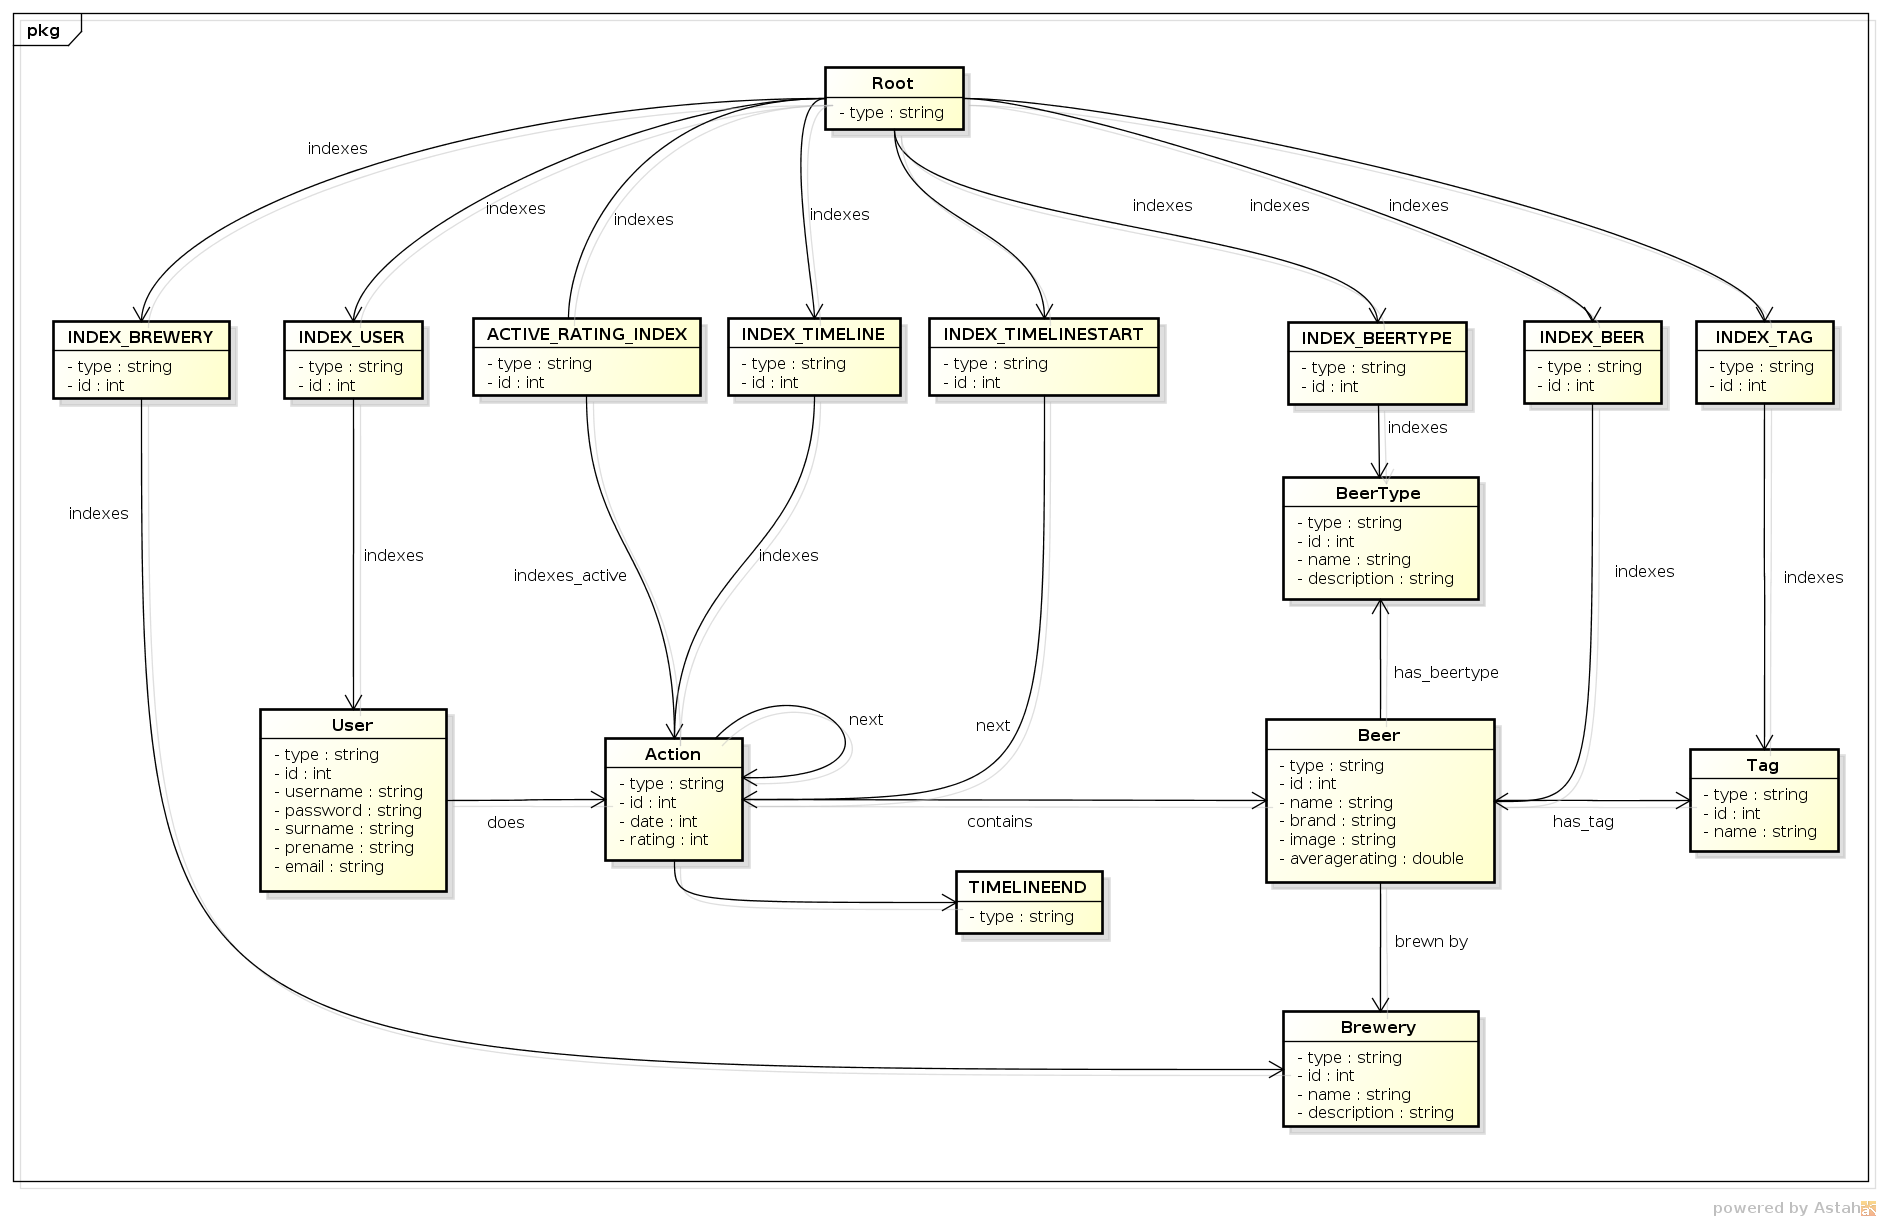
\includegraphics[height=0.9\textwidth,angle=90]{Database_Design_Graph.png}
	\caption{Allgemeines Datenbankdesign}
	\label{fig:database_design}
\end{figure}

\begin{figure}[H]
	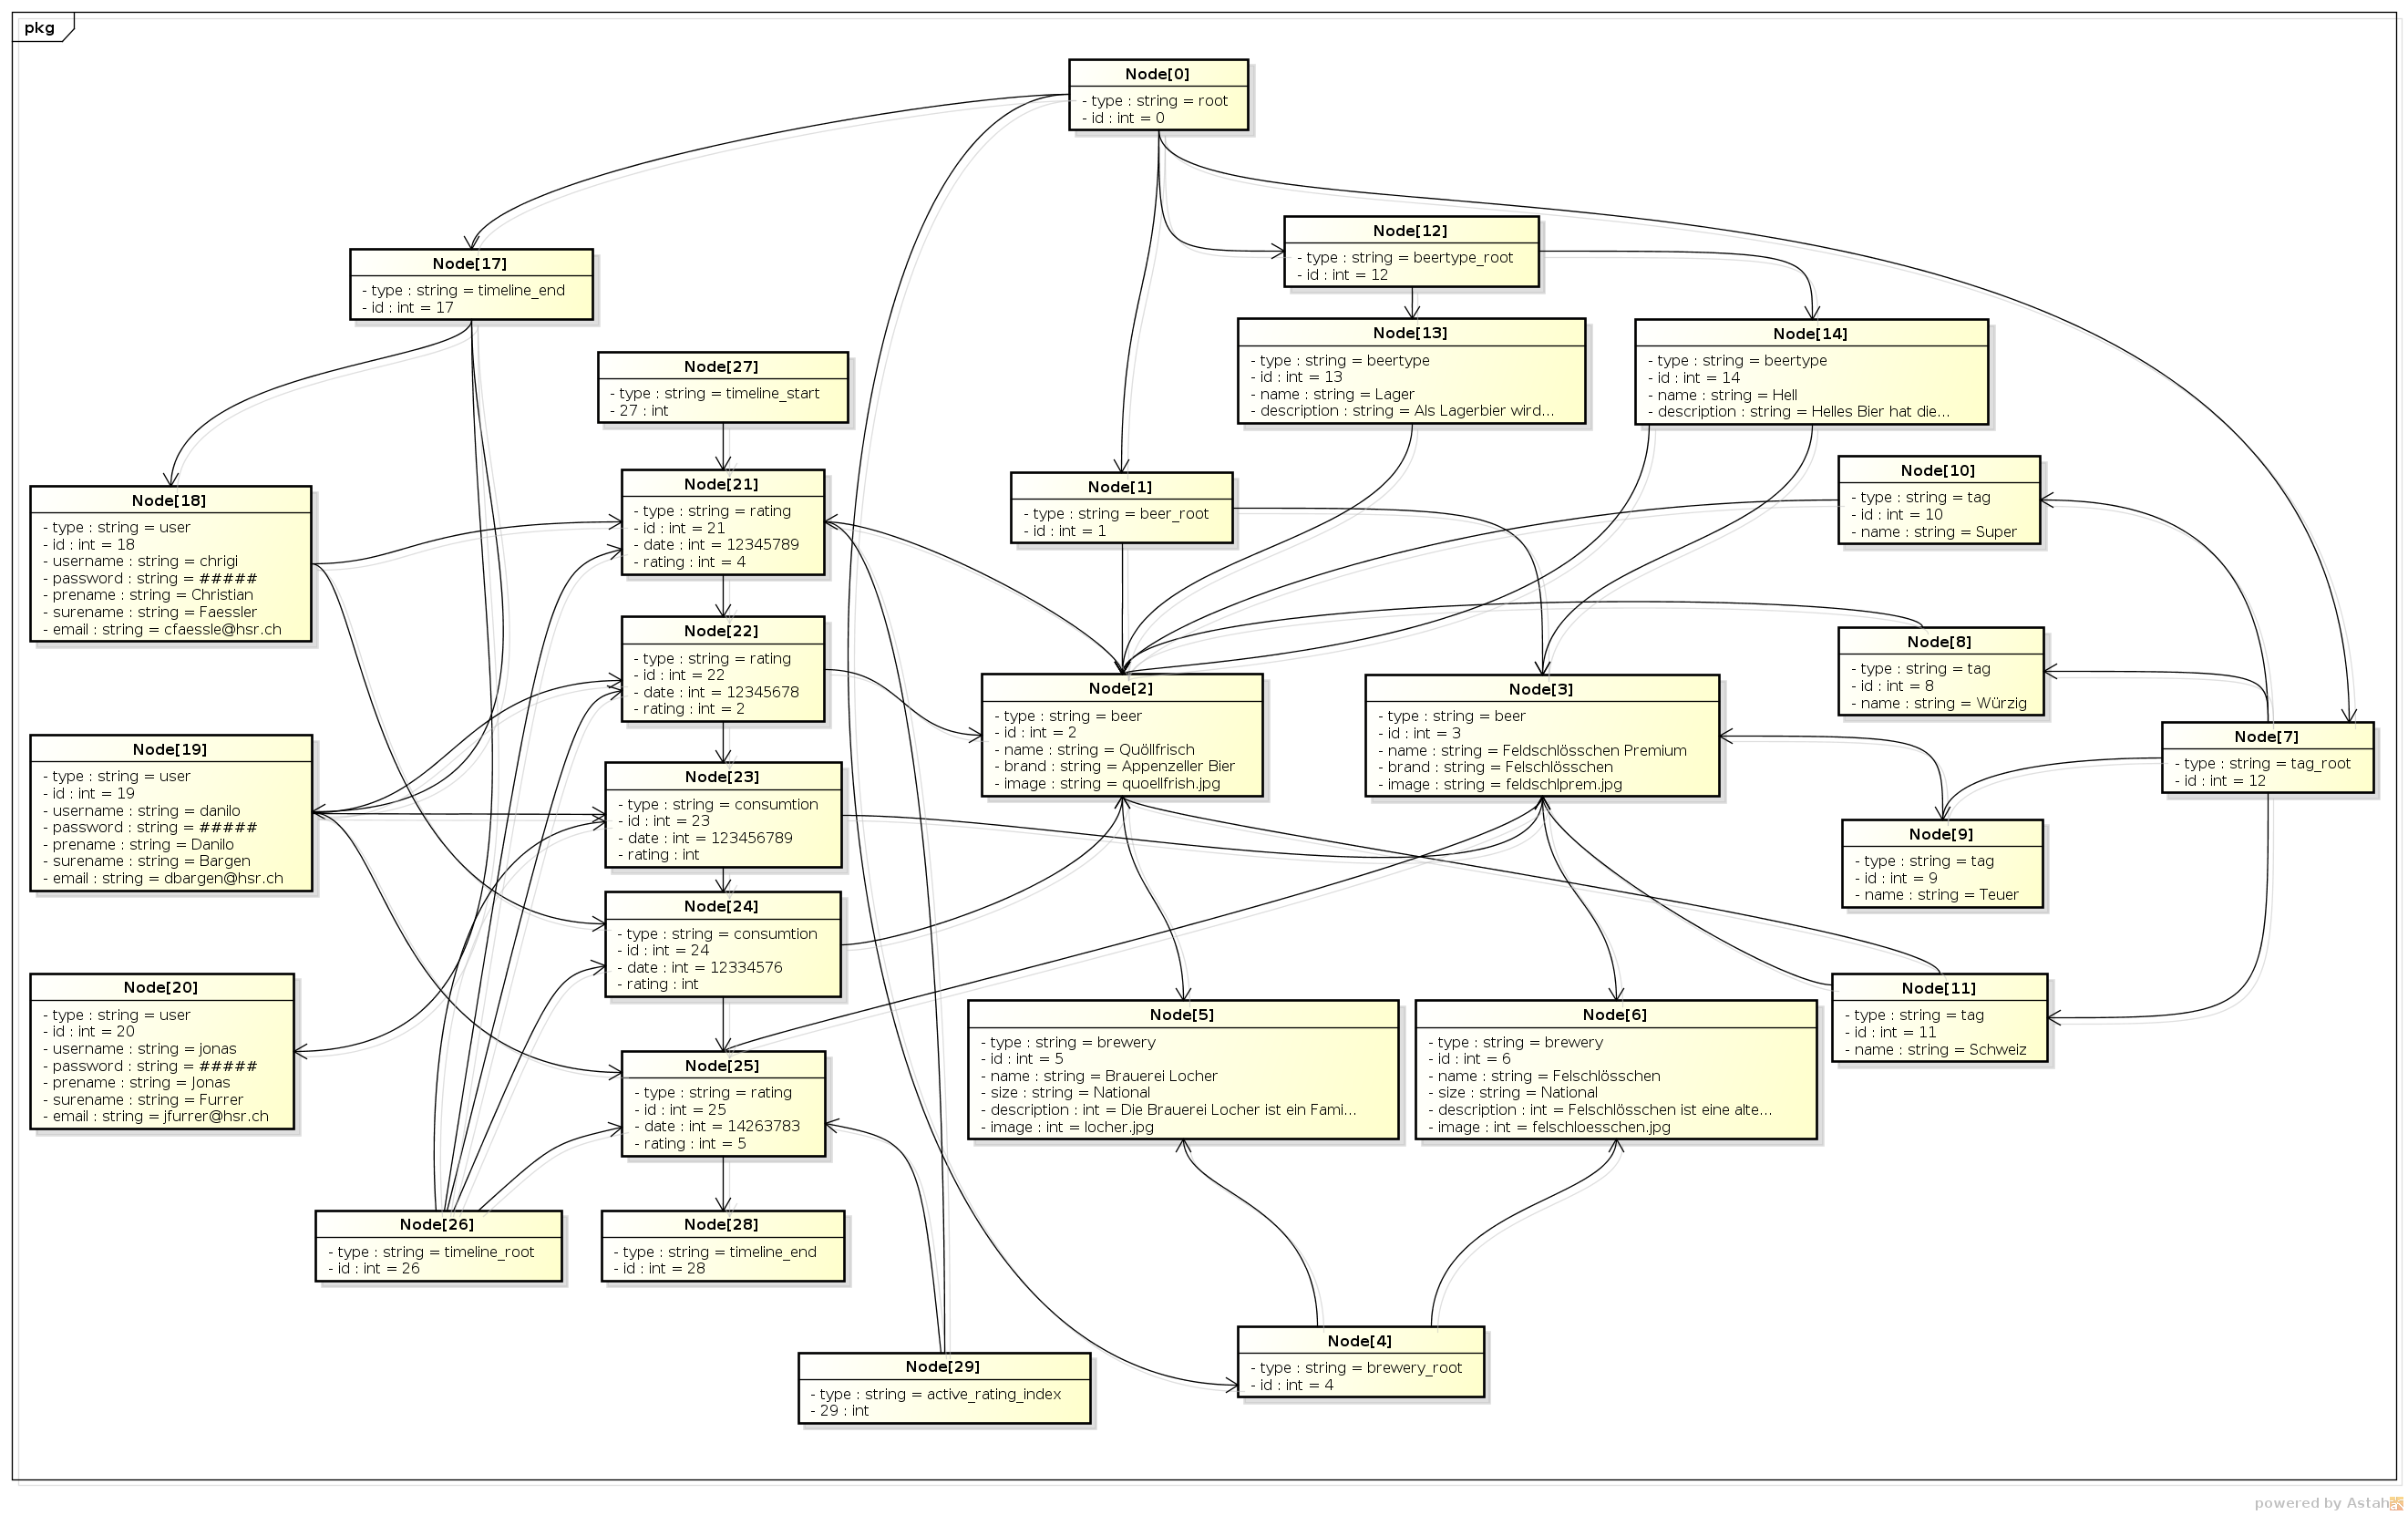
\includegraphics[height=\textwidth,angle=90]{Database_Example.png}
	\caption{Datenbank Beispielfall}
	\label{fig:database_design_example}
\end{figure}


\section{Grössen und Leistung}

Im Rahmen dieses Projektes ist das System und die serverseitige Umgebung für den
Einsatz mit bis zu 50 Benutzern, rund 100 Bieren und 20 Brauereien ausgelegt.
Es sollte aber skalierbar sein, so dass mit besserer Serverumgebung erheblich
mehr Benutzer bedient werden könnten.

Die Architektur wird so ausgelegt, dass so wenig Rechenleistung wie möglich auf der Clientseite
benötigt wird. Das heisst, sämtliche Logik und Aufbereitung der Daten wird auf der Serverseite
implementiert. Da clientseitig die Unterschiede in der verwendeten Hardware sehr gross sein
können (Smartphones, Tablets, Netbooks), können keine einheitlichen Anforderungen zur
Rechenkapazität auf den Geräten gestellt werden. Desweiteren muss heutzutage bei der Entwicklung
von Mobile Apps stark auf den Energieverbrauch geachtet werden. Mit der zentralisierten Ausführung
rechenintensiver Aufgaben sind die verfügbaren Ressourcen bekannt und die Software kann entsprechend
adäquat entwickelt werden.


\end{document}
